\documentclass[10pt, xcolor=x11names, compress]{beamer}
\usetheme{progressbar}
\progressbaroptions{headline=sections,titlepage=normal,frametitle=normal}

\setbeamertemplate{navigation symbols}{}

\usepackage{iwona} 
\usepackage{alltt}
\usepackage{amsmath,amsfonts, amssymb, amscd}
\usepackage{hyperref}
\usepackage{setspace}
\usepackage{wasysym}

\usepackage{calc}
\usepackage[overlay,absolute]{textpos}
\TPGrid[5mm,5mm]{20}{20}

\renewcommand{\Re}{\operatorname{Re}}
\renewcommand{\Im}{\operatorname{Im}}
\newcommand{\debye}{\operatorname{debye}}

\newcommand{\chik}{$\chi(k)$}
\newcommand{\chir}{$|\tilde{\chi}(R)|$}


\newcommand{\file}[1]{{\color{Firebrick4}\texttt{`#1'}}}
\newcommand{\multiple}{{\color{Orange2}\textsl{multiple}}}


\newcommand{\atoms}  {{\color{Brown4}\textsc{atoms}}}
\newcommand{\feff}   {{\color{Brown4}\textsc{feff}}}
\newcommand{\ifeffit}{{\color{Brown4}\textsc{ifeffit}}}
\newcommand{\athena} {{\color{Brown4}\textsc{athena}}}
\newcommand{\artemis}{{\color{Brown4}\textsc{artemis}}}

\newcommand{\ybco}{YBa$_2$Cu$_3$O$_7$}
\newcommand{\eto}{EuTiO$_3$}
\newcommand{\bton}{BaTaO$_2$N}
\newcommand{\ufivemineral}%
{U$^{\mathrm{V}}$(H$_2$O)$_2$(U$^{\mathrm{VI}}$O$_2$)$_2$O$_4$(OH)+4$\cdot$H$_2$O}

\renewenvironment<>{center}
{\begin{actionenv}#1\begin{originalcenter}}
{\end{originalcenter}\end{actionenv}}



\mode<presentation>
%\mode<beamer>

\title{Interpreting XANES Data}



\author{Bruce Ravel}
\institute[NIST]{
  Synchrotron Methods Group, Ceramics Division\\%
  Materials Measurement Laboratory\\%
  National Institute of Standards and Technology\\%
  \&\\%
  Local Contact, Beamline X23A2\\%
  National Synchrotron Light Source\\[3ex]~}

\date[1$^{\mathrm{st}}$ ASEAN XAS]{1$^{\mathrm{st}}$ ASEAN Workshop on
  X-ray Absorption Spectroscopy\\Synchrotron Light Research
  Institute\\Nakhon Ratchasima, Thailand \\29--31 July 2010}

% \logo{
\includegraphics[width=1.0cm]{images/ankaxas_black.png}}

\begin{document}
\begin{frame}
  \titlepage
\end{frame}

\begin{frame}
  \frametitle{Copyright}
  \tiny

  This document is copyright \copyright 2007-2010 Bruce Ravel.

  \begin{center}
    
\includegraphics[width=1.0cm]{images/somerights20}
  \end{center}

  This work is licensed under the Creative Commons
  Attribution-ShareAlike License.  To view a copy of this license,
  visit \href{http://creativecommons.org/licenses/by-sa/3.0/}
  {\color{Purple4}\texttt{http://creativecommons.org/licenses/by-sa/3.0/}}
  or send a letter to Creative Commons, 559 Nathan Abbott Way,
  Stanford, California 94305, USA.

  \begin{description}
  \item[You are free:] %
    \begin{itemize}
    \item \textbf{to Share} --- to copy, distribute, and transmit the work
    \item \textbf{to Remix} --- to adapt the work
    \end{itemize}
  \item[Under the following conditions:] %
    \begin{itemize}
    \item Attribution. You must attribute the work in the manner
      specified by the author or licensor (but not in any way that
      suggests that they endorse you or your use of the work).
    \item Share Alike. If you alter, transform, or build upon this
      work, you may distribute the resulting work only under the same,
      similar or a compatible license.
    \item Any of these conditions can be waived if you get permission
      from the author.
    \end{itemize}
  \end{description}
  \begin{itemize}
  \item For any reuse or distribution, you must make clear to others
    the license terms of this work. The best way to do this is with a
    link to the URL for this document.
  \item Any of the above conditions can be waived if you get
    permission from the copyright holder.
  \item Nothing in this license impairs or restricts the author's
    moral rights.
  \end{itemize}

  Your fair dealing and other rights are in no way affected by the
  above.  This is a human-readable summary of the Legal Code (the full
  license).


\end{frame}

%%% Local Variables:
%%% mode: latex
%%% TeX-master: "pimst2"
%%% End:


%\mode<handout>{\frame{\tableofcontents}}

%% \section*{Outline}
%% \begin{frame}
%%   \tableofcontents
%% \end{frame}


\begin{frame}
  \frametitle{Acknowledgment}

  This talk is heavily influenced by Simon Bare's excellent XANES talk
  at the 2008 APS XAFS Summer School.  See
  \href{http://xafs.org/Workshops/APS2008}
  {http://xafs.org/Workshops/APS2008}.
\end{frame}

\section[Overview]{Overview}

\begin{frame}
  \frametitle{Acronyms}
  \begin{description}
  \item[XANES] \alert{X}-ray \alert{A}bsorption
    \alert{N}ear-\alert{E}dge \alert{S}tructure
  \item[NEXAFS] \alert{N}ear-\alert{E}dge \alert{X}-ray
    \alert{A}bsorption \alert{F}ine \alert{S}tructure
  \end{description}

  \bigskip

  XANES and NEXAFS are \emph{exactly} the same thing.  Historically,
  the soft X-ray community says ``NEXAFS'' while the hard X-ray
  community says ``XANES''.

  \bigskip

  Both acronyms refer to the portion of the XAS (\alert{X}-ray
  \alert{A}bsorption \alert{S}pectroscopy) measurement in the vicinity
  of the absorption edge.

  \bigskip

  The \alert{E}xtended \alert{X}-ray \alert{A}bsorption \alert{F}ine
  \alert{S}tructure is oscillatory data extending hundreds of volts
  above the edge.
\end{frame}

\begin{frame}
  \frametitle{Some vocabulary}

  Words commonly used to describe specific parts of the XANES spectrum.

  \begin{columns}[T]
    \begin{column}{0.5\linewidth}
      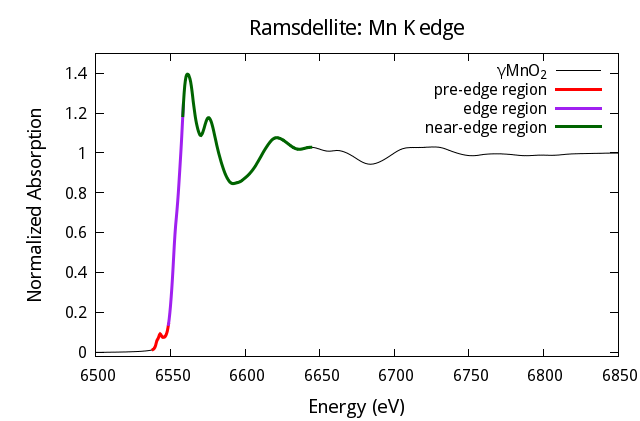
\includegraphics[width=\linewidth]{images/rams/ramsdellite.png}

      \small

      \begin{description}[edge]
      \item[{\color{red}pre-edge}] Small (or large, certainly
        meaningful!) features between the Fermi energy and the
        threshold
      \item[{\color{DarkOrchid2}edge}] The main rising part of XAS spectrum
      \item[{\color{Green4}near-edge}] Characteristic features above the edge
      \end{description}
    \end{column}    
    \begin{column}{0.5\linewidth}
      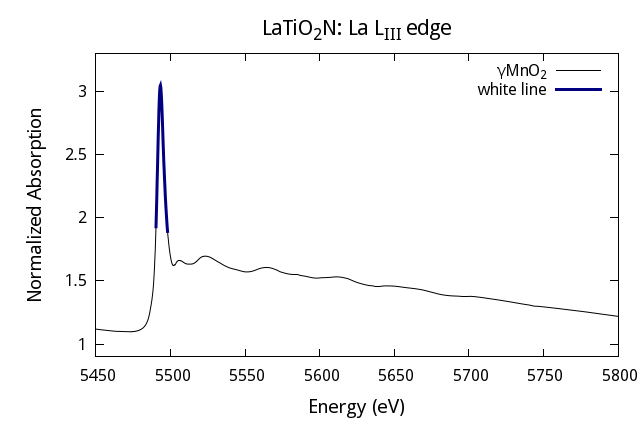
\includegraphics[width=\linewidth]{images/ltno/ltno.png}

      \begin{description}[wh]
      \item[{\color{Blue3}white line}] Large, prominent peak just
        above the edge, particularly in L or M edge spectra
      \end{description}
    \end{column}    
  \end{columns}
\end{frame}

\begin{frame}
  \frametitle{XANES Publications}

  Interest in XANES and its interpretation has grown steadily over the
  the last 3 decades as XAS has become more available and adopted by
  more scientific disciplines.

  \begin{center}
    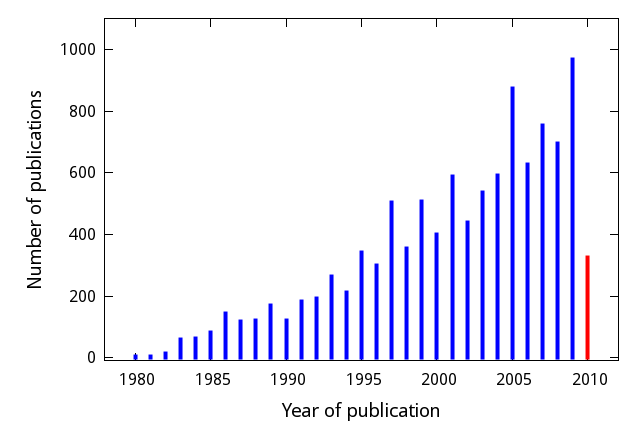
\includegraphics[width=0.75\linewidth]{images/pubs/xanes_pubs.png}

    \tiny Results of a search at \href{http://pcs.isiknowledge.com/}
    {\color{Purple4}ISI Web of Knowledge} for the word ``XANES'':
  \end{center}
\end{frame}

\section[Information]{Information Content of XANES}

\subsection{Speciation}
\begin{frame}
  \frametitle{Speciation at a glance: Coordination}

  Here is Cr K edge data for {\color{Blue3}tetragonally coordinated,
    hexavalent K$_2$Cr$^{\textrm{VI}}$O$_7$} and
  {\color{Red2}hexagonally coordinated, trivalent
    Cr$^{\textrm{III}}_2$O$_3$}.  Trivalent Cr is insoluble and
  non-toxic.  Hexavalent Cr is readily soluble and highly toxic.

  \begin{columns}
    \begin{column}{0.7\linewidth}
      \begin{center}
        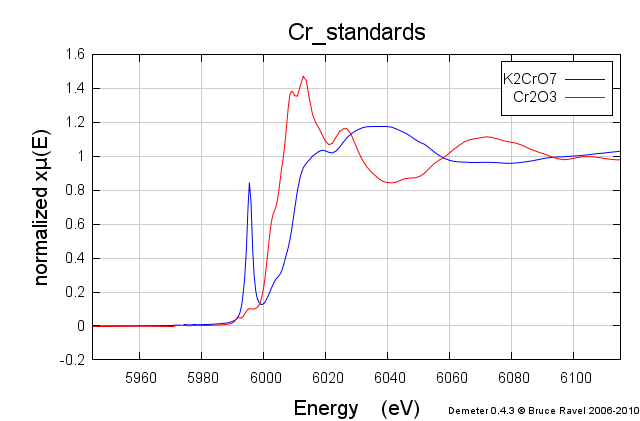
\includegraphics[width=0.9\linewidth]{images/Cr/Cr.png}
      \end{center}
    \end{column}
    \begin{column}{0.3\linewidth}
      \begin{center}
        {\color{Blue3}K$_2$CrO$_7$}\\
        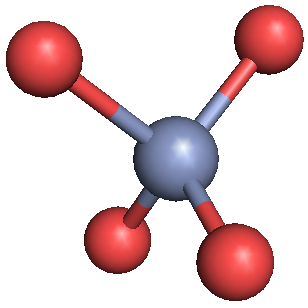
\includegraphics[width=0.5\linewidth]{images/Cr/K2CrO7.png}\\[2ex]
        {\color{Red2}Cr$_2$O$_3$}\\
        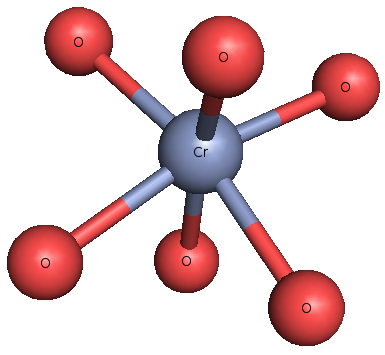
\includegraphics[width=0.5\linewidth]{images/Cr/Cr2O3.png}
      \end{center}
    \end{column}
  \end{columns}

  \smallskip

  It is very easy to tell ``good'' Cr from ``bad'' Cr in a XANES
  measurement.

  \begin{textblock*}{0.6\linewidth}(0pt,20\TPVertModule) 
    \tiny
    data from 
    \href{http://cars9.uchicago.edu/~newville/ModelLib/search.html}
    {\texttt{http://cars9.uchicago.edu/\char126newville/ModelLib/search.html}}
  \end{textblock*}
\end{frame}

\begin{frame}
  \frametitle{Speciation at a glance: Crystallinity}

  SiO$_2$ is found in two forms$^\ast$ under standard conditions:
  {\color{Blue3}crystalline (the mineral quartz)} and {\color{Red2}amorphous
  (common glass)}.

  \begin{center}
    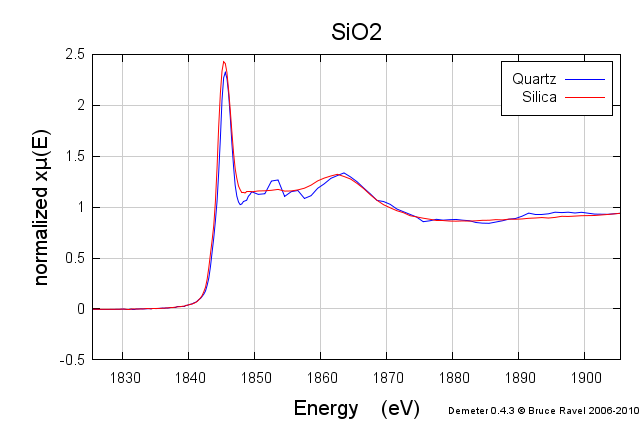
\includegraphics[width=0.7\linewidth]{images/SiO2.png}
  \end{center}

  Again, these are readily distinguished by a XANES measurement.

  \begin{textblock*}{0.55\linewidth}(0pt,20\TPVertModule) 
    \tiny
    $^\ast$Wikipedia identifies 14 other metastable, high-T,
    or high-P forms of SiO$_2$.
  \end{textblock*}
\end{frame}

\begin{frame}
  \frametitle{Speciation at a glance: Oxidation}
  
  \begin{columns}
    \begin{column}{0.4\linewidth}
      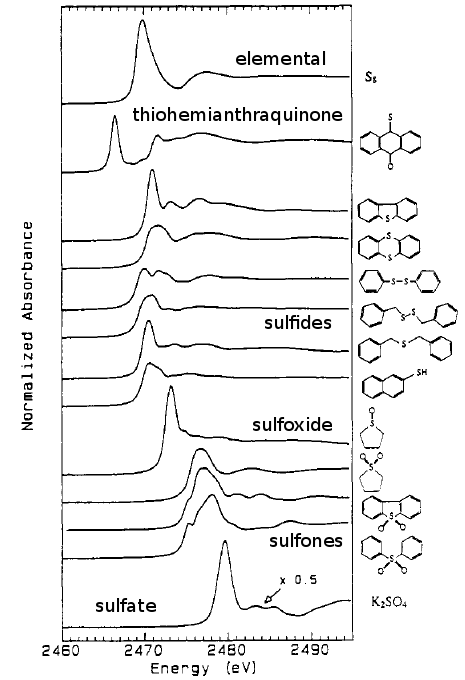
\includegraphics[width=\linewidth]{images/S.png}
    \end{column}
    \begin{column}{0.6\linewidth}
      \begin{itemize}
      \item There is an 11\,eV shift from S$^{2-}$ to S$^{6+}$ with
        lots of variation among species.
      \item S speciation is of importance across a broad range of
        disciplines, including life science, catalysis, petroleum
        science, photovoltaics, environmental science and more.
      \item P and Cl are similarly rich in their XAS.
      \item XAS of S, P, and Cl are a particular strength of BL8
        $\ddot\smile$
      \end{itemize}

    \end{column}    
  \end{columns}

  \begin{textblock*}{0.5\linewidth}(0pt,19\TPVertModule) 
    \tiny
    \textit{Sulfur K-edge x-ray absorption spectroscopy of petroleum
    asphaltenes and model compounds},
    G.N.\ George, M.L.\ Gorbaty,
    J.\ Am.\ Chem.\ Soc.\ (1989) \textbf{111}:9, 3182~
    \href{http://dx.doi.org/10.1021/ja00191a012}
    {\color{Purple4}DOI: 10.1021/ja00191a012}
  \end{textblock*}
\end{frame}

\subsection{Oxidation}
\begin{frame}
  \frametitle{Oxidation and edge position}

  \small

  \begin{columns}
    \begin{column}{0.4\linewidth}
      There is a relationship between formal valence of a metal and the
      position of the edge in the XANES spectrum.  Here is Re metal along
      with 4+, 6+, and 7+ oxides of Re.

      \smallskip

      The shift to higher energy is, to first order, a Coulomb effect.
      Less charge on the atom means less screening of the core.
    \end{column}
    \begin{column}{0.6\linewidth}
      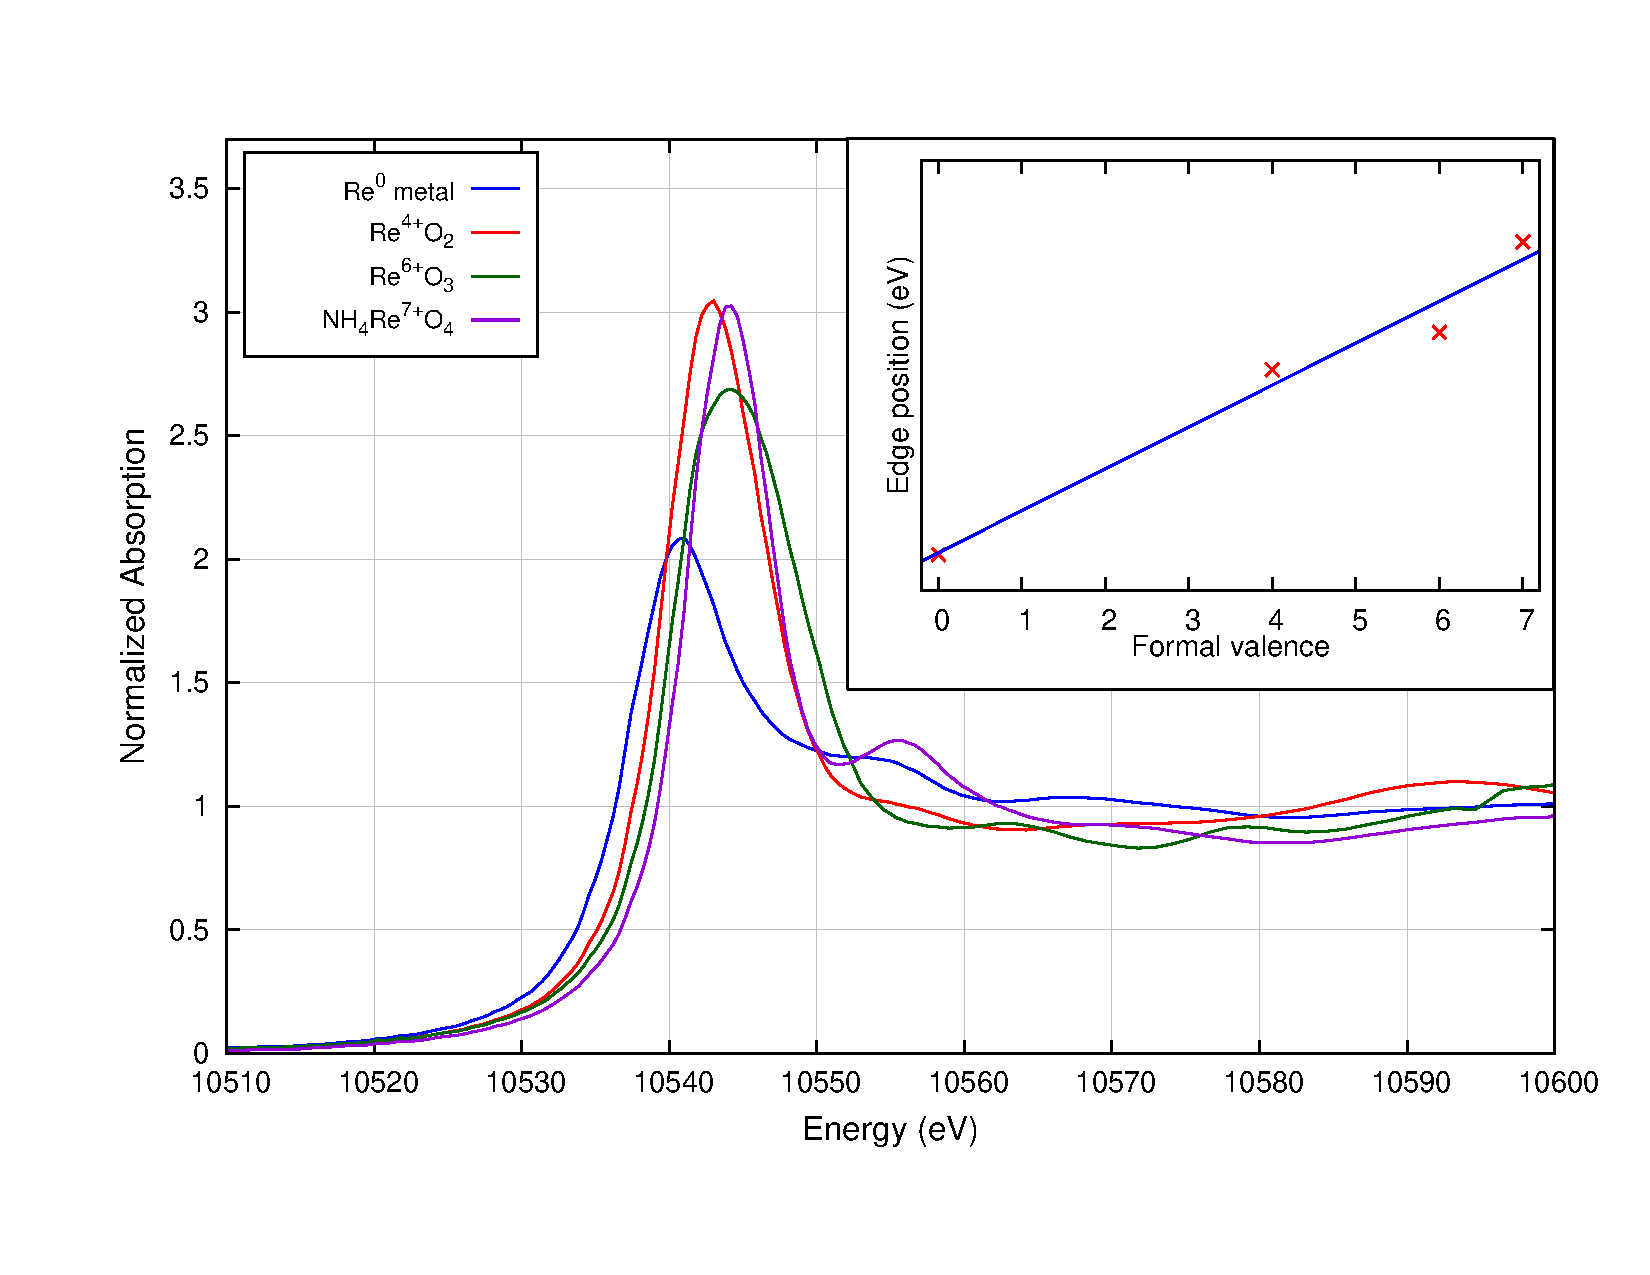
\includegraphics[width=\linewidth]{images/Re_valence.pdf}
    \end{column}
  \end{columns}
  

  Some more examples:
  \begin{description}[Mo]
  \item[Mo] S.P.\ Cramer et al. J. Am. Chem. Soc., (1976) \textbf{98}:5, pp
    1287
  \item[V] J.\ Wong et al. Phys. Rev. B\textbf{30}, 5596--5610 (1984) 
  \end{description}

    
  \begin{textblock*}{0.5\linewidth}(0pt,19\TPVertModule) 
    \tiny
    \textit{Simultaneous XAFS measurements of multiple samples},
    B.\ Ravel, C.\ Scorzato, D.P.\ Siddons, S.D.\ Kelly and S.R.\ Bare,
    J. Synchrotron Rad. (2010) \textbf{17}, 380-385
    \href{http://dx.doi.org/10.1107/S0909049510006230}
    {\color{Purple4}doi:10.1107/S0909049510006230}
  \end{textblock*}
\end{frame}

\begin{frame}
  \frametitle{Mixed phases}

  \begin{columns}
    \begin{column}{0.4\linewidth}
      Here we see {\color{Blue3}trivalent V$_2$O$_3$},
      {\color{Red2}pentavalent V$_2$O$_5$} and an
      {\color{Green4}unknown Vanadium compound} plotted together.
    \end{column}
    \begin{column}{0.6\linewidth}
      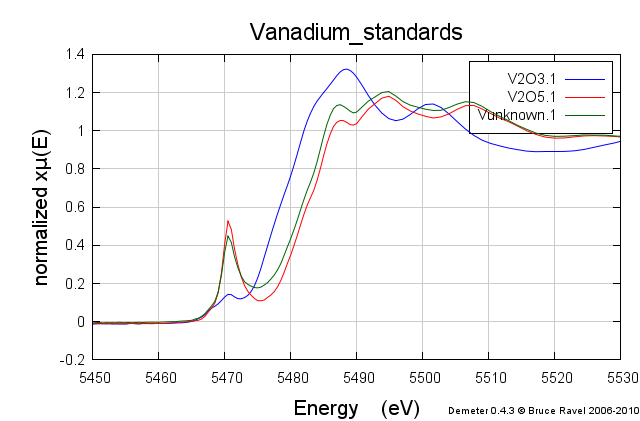
\includegraphics[width=\linewidth]{images/V.png}
    \end{column}
  \end{columns}

  \bigskip
  
  Like in the Cr example, we see a distinct difference between
  6-coordinated and 4-coordinated V.

  \bigskip

  Our unknown is partially reduced, as can be seen by the reduction in
  pre-edge peak and the left-ward shift of the main edge.

  \bigskip

  Later we will discuss ways of determining the content of the
  unknown.
\end{frame}

\begin{frame}
  \frametitle{Evolution of redox state}

  The edge features are often large enough that their evolution can be
  measured in an \textit{in situ} experiment.
  \begin{columns}
    \begin{column}{0.4\linewidth}
      Here we see the kinetics of $\mathrm{Cr}^{III}\rightarrow
      \mathrm{Cr}^{VI}$ oxidation by Mn oxide over the course of four
      minutes of reaction time.  Each scan was measured in 3 second.
    \end{column}
    
    \begin{column}{0.6\linewidth}
      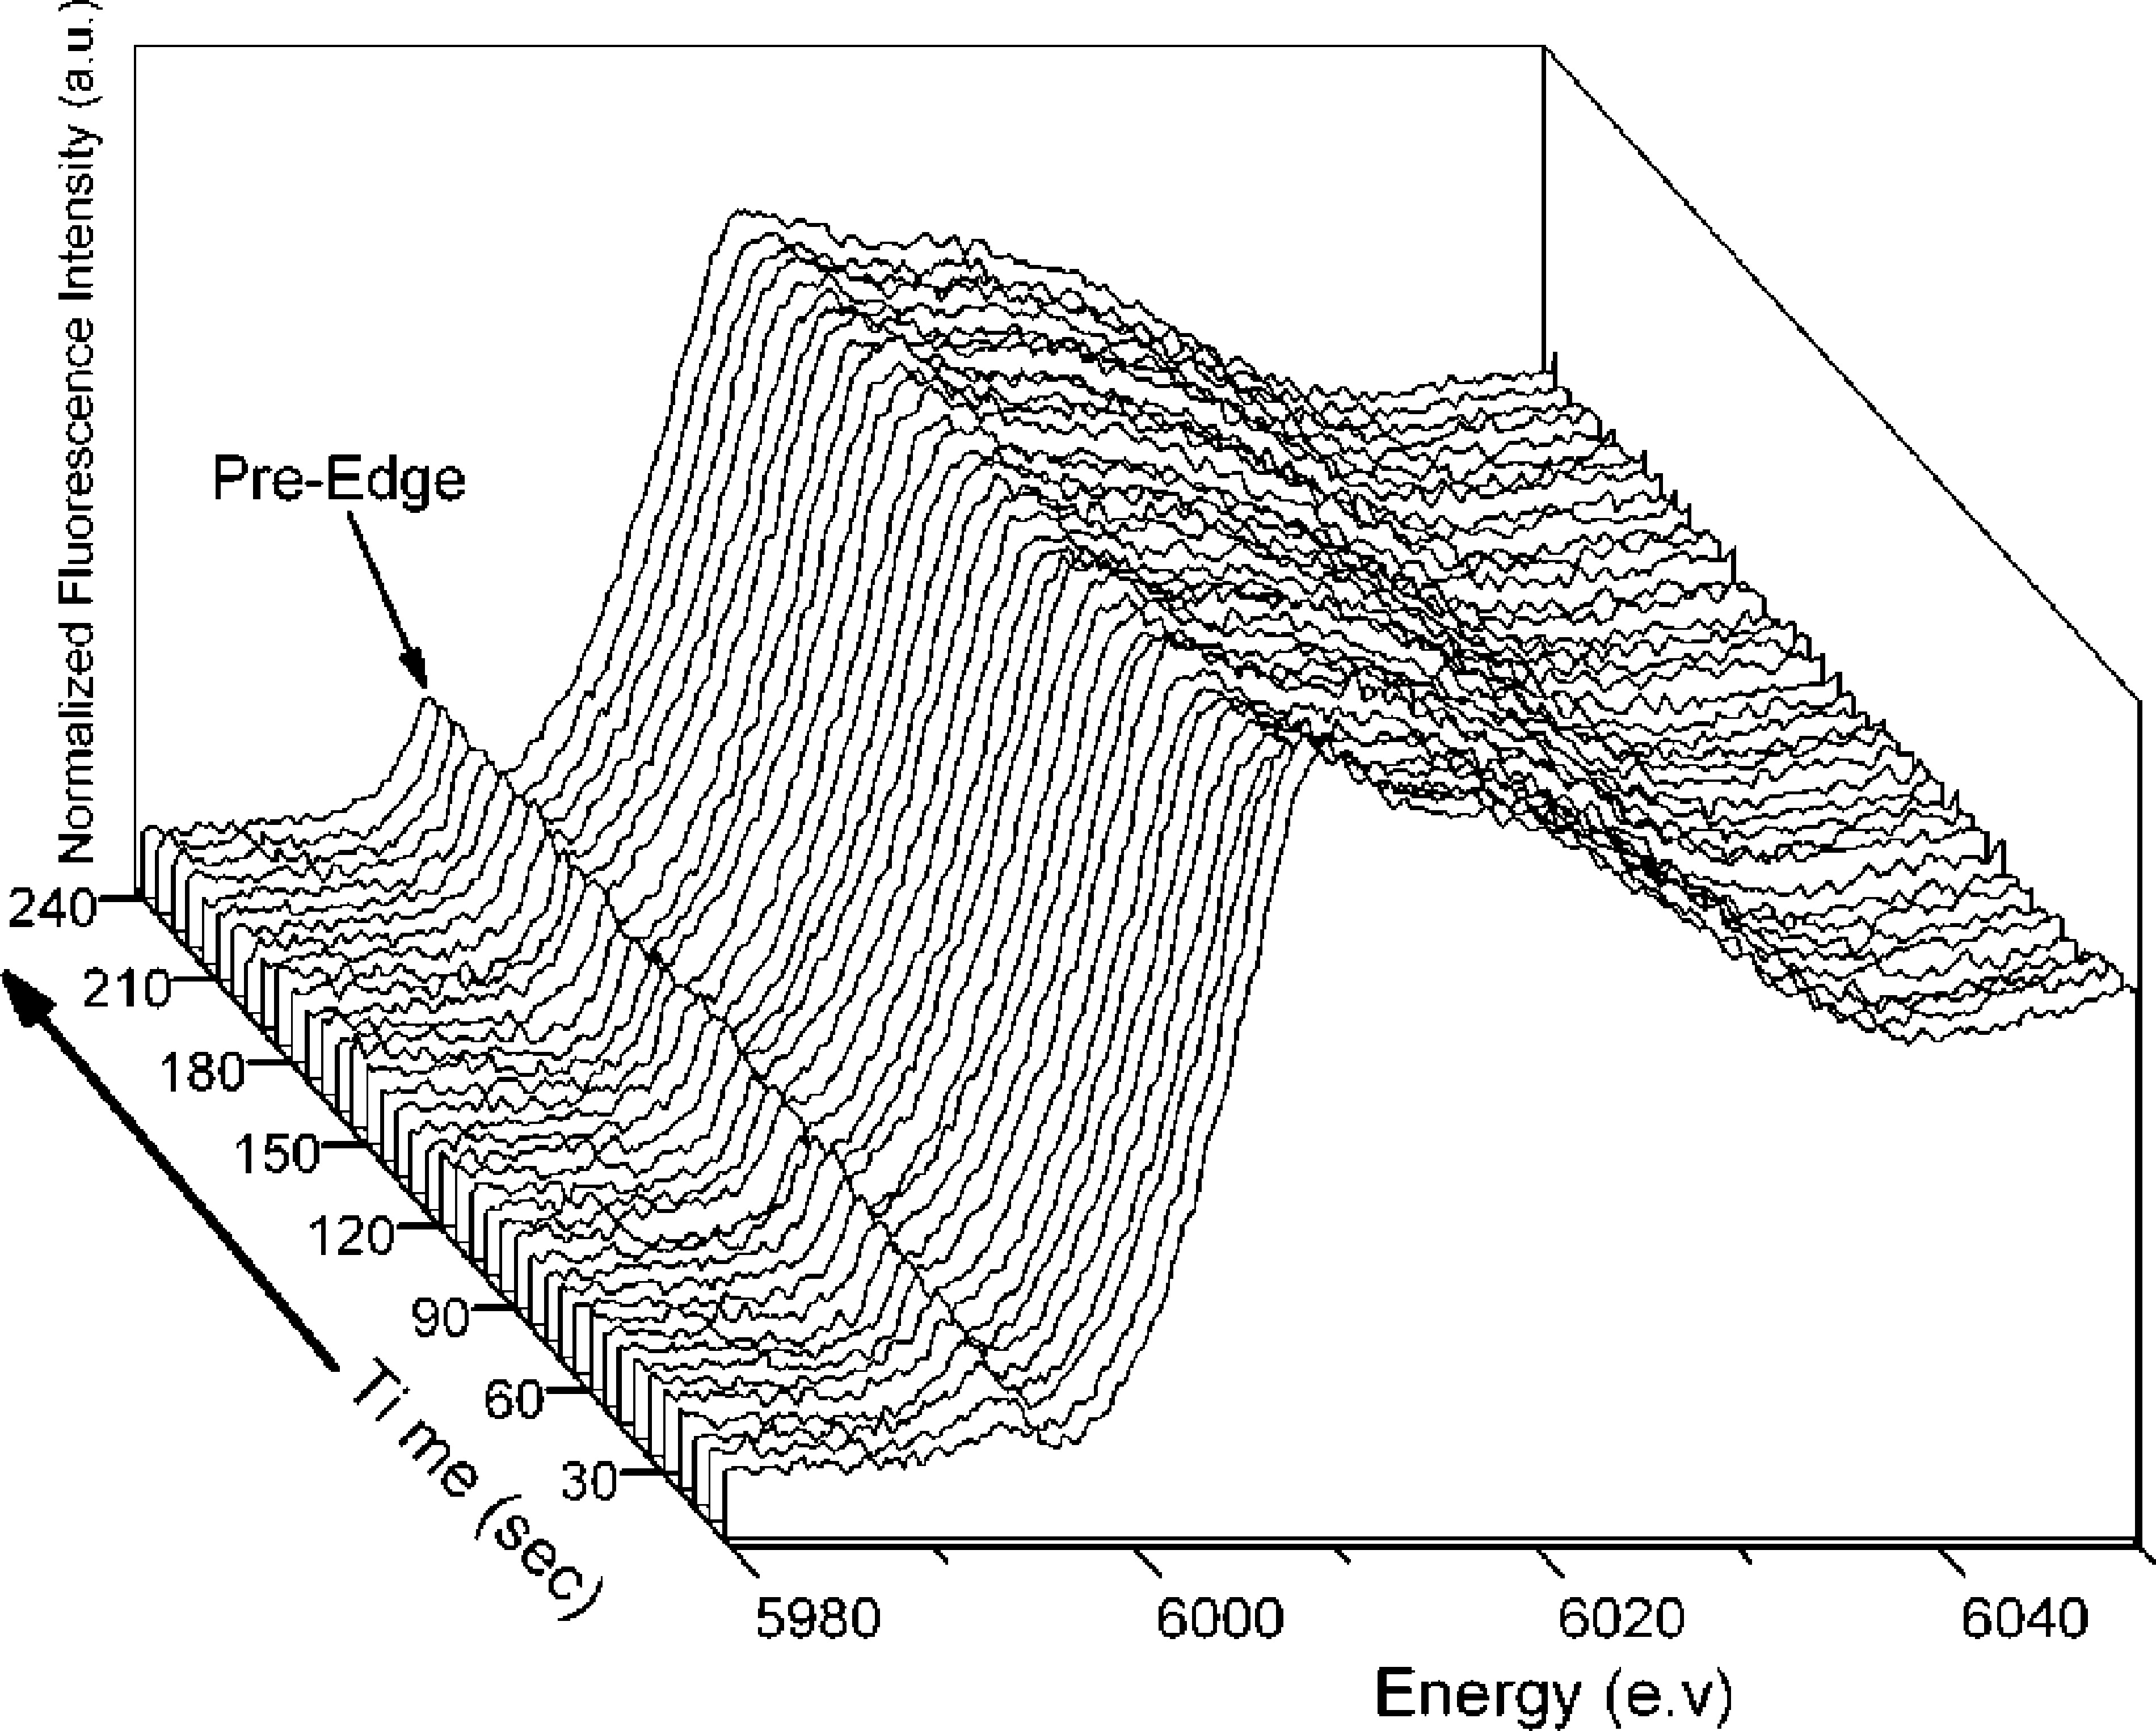
\includegraphics[width=\linewidth]{images/cr_reduction.png}
    \end{column}
  \end{columns}

  The \textit{in situ} experiment could involve a chemical reaction, a
  change in temperature, electrochemical cycling, and so on.

  \begin{textblock*}{0.5\linewidth}(0pt,18.5\TPVertModule)
    \tiny%
    \textit{Kinetics of Chromium(III) Oxidation by Manganese(IV)
      Oxides Using Quick Scanning X-ray Absorption Fine Structure
      Spectroscopy (Q-XAFS)}, G.\ Landrot, M.\ Ginder-Vogel,
    and D.L.\ Sparks, Environ. Sci. Technol., (2010) \textbf{44}:1, pp
    143-149 \href{http://dx.doi.org/10.1021/es901759w}
    {\color{Purple4}DOI: 10.1021/es901759w} 
  \end{textblock*}
\end{frame}

\subsection{Ligands}
\begin{frame}
  \frametitle{Ligands}


  \begin{columns}
    \begin{column}{0.6\linewidth}
      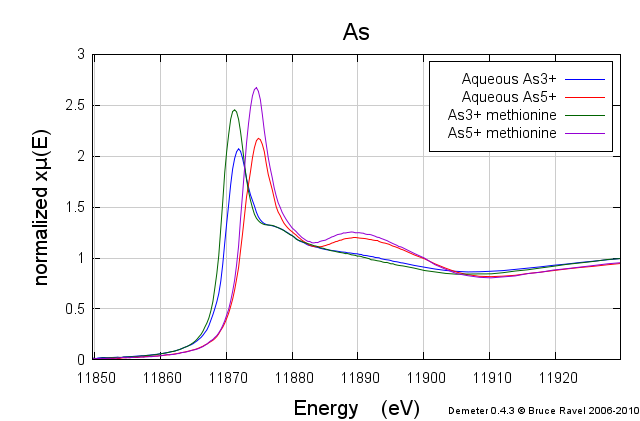
\includegraphics[width=0.9\linewidth]{images/As.png}\\
      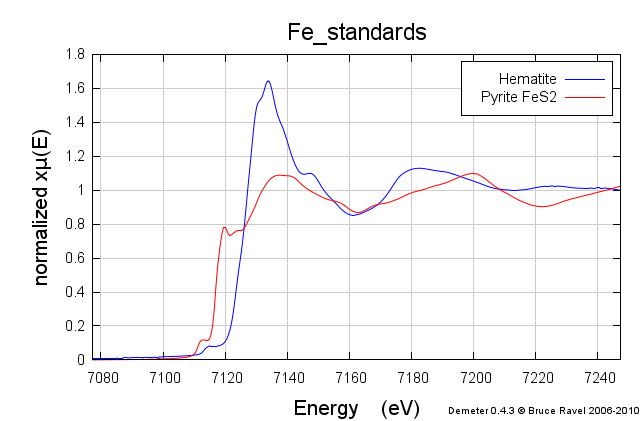
\includegraphics[width=0.9\linewidth]{images/Fe.png}
    \end{column}
    \begin{column}{0.4\linewidth}
      We see a significant edge shift between {\color{Blue3}aqueous
        As$^{3+}$} and {\color{Red2}aqueous As$^{5+}$}, as we expect.
      Note that the {\color{Green4}As$^{3+}$} and
      {\color{Purple4}As$^{5+}$} methionine solutions are similar, but
      shifted to lower energy.

      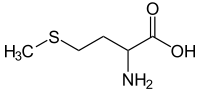
\includegraphics[width=0.7\linewidth]{images/methionine.png}

      The same shift is seen between divalent {\color{Blue3} hematite
        (Fe$_2$O$_3$)} and the nominally divalent {\color{Red2}pyrite
        (FeS$_2$)}.
    \end{column}
  \end{columns}
  \begin{columns}
    \begin{column}{0.6\linewidth}
    \end{column}
    \begin{column}{0.4\linewidth}
    \end{column}
  \end{columns}
\end{frame}


\section[Measure]{Measuring XANES Data}

\begin{frame}
  \frametitle{Sample preparation}

  Sample preparation for XANES is fairly forgiving and usually pretty
  easy.  Here are three examples:

  \smallskip

  \begin{columns}
    \begin{column}{0.5\linewidth}
      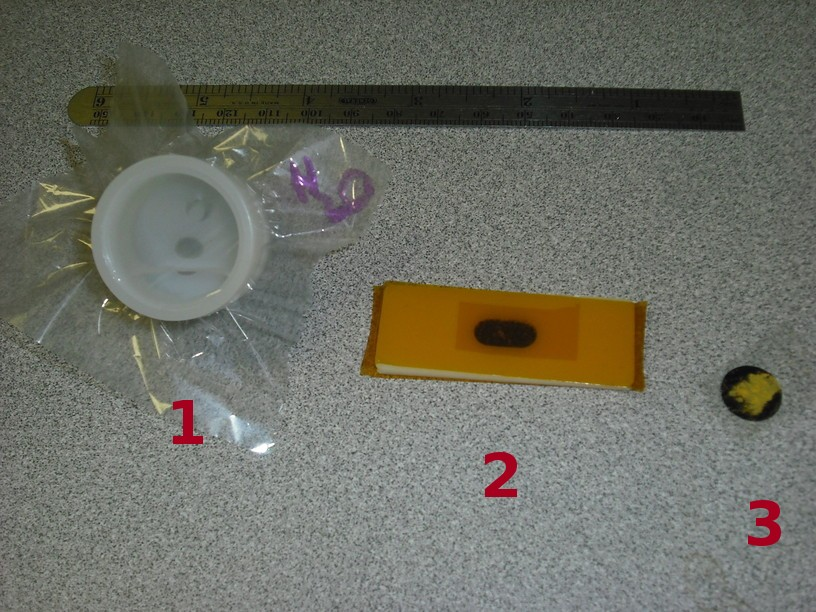
\includegraphics[width=\linewidth]{images/samples.jpg}
    \end{column}
    \begin{column}{0.5\linewidth}
      \begin{enumerate}
      \item A Spex XRF vessel is great for solution samples.
      \item A simple frame and tape is fine for powders.
      \item A carbon tape with powder sprinkled on is useful for lower
        energy edges.
      \end{enumerate}

    \end{column}
  \end{columns}

  \bigskip

  Ideally, the sample is homogeneous, but in practice almost anything
  can be used.

  \smallskip

  For example, cultural heritage samples are often placed \textit{as
    is} in the beam.
\end{frame}

\begin{frame}
  \frametitle{Sensible scan parameters}
  \begin{itemize}
  \item Through the edge, the measurement grid must be very fine to
    adequately measure the quickly changing data.
  \item If using a third derivative analysis (see the reference
    below), your data grid through the edge must be much finer than
    the experimental resolution.
  \item Enough of the pre-edge and post-edge must be measured to do a
    good job normalizing the data.
  \end{itemize}

  \begin{columns}
    \begin{column}{0.5\linewidth}
      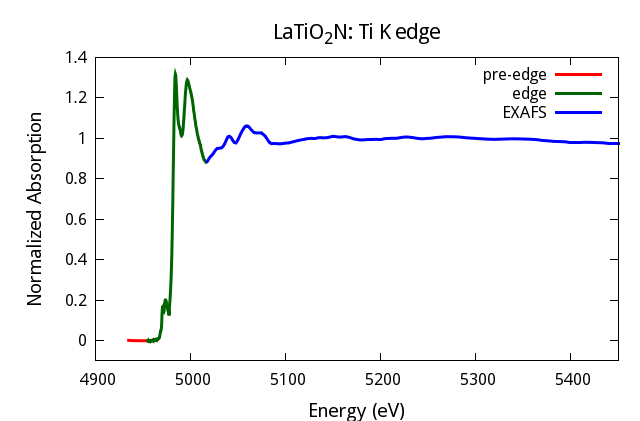
\includegraphics[width=\linewidth]{images/scan_params/scan_params.png}
    \end{column}
    \begin{column}{0.5\linewidth}
      \begin{tabular}[h]{rl}
        region & step size\\
        \hline
        \color{Red2}pre-edge & \color{Red2}5\,eV\\
        \color{Green4}edge   & \color{Green4}0.25\,eV\\
        \color{Blue3}EXAFS   & \color{Blue3}$0.05\,\textrm{\AA}^{-1}$\\
      \end{tabular}

      \smallskip

      \small%
      {\color{Green4}0.25\,eV} is reasonable for $\sim$5\,keV.  A
      larger step is OK at higher energy, a smaller step might be
      needed for lower energies.
    \end{column}
  \end{columns}

  \begin{textblock*}{0.5\linewidth}(0pt,19\TPVertModule) 
    \tiny
    \textit{Sulfur K-edge x-ray absorption spectroscopy of petroleum
    asphaltenes and model compounds},
    G.N.\ George, M.L.\ Gorbaty,
    J.\ Am.\ Chem.\ Soc.\ (1989) \textbf{111}:9, 3182~
    \href{http://dx.doi.org/10.1021/ja00191a012}
    {\color{Purple4}DOI: 10.1021/ja00191a012}
  \end{textblock*}
\end{frame}

\begin{frame}
  \frametitle{Self-absorption}

  As $\mu(E)$ changes through the edge and fine-structure, the
  penetration depth of the sample changes, thus changing the sample
  volume contributing to the fluorescence measurement.  This has the
  effect of attenuating the XAS.\\[-0.5ex]
  \href{http://xafs.org/Experiment/OverAbsorption?action=AttachFile&do=get&target=overabsorption.pdf}{\color{Purple4}\tiny
    (See A. Manceau, M.A. Marcus, N. Tamura (2002) Reviews in
    Mineralogy and Geochemistry, 49, 341-428.)}

  \begin{columns}[T]
    \begin{column}{0.5\linewidth}
      \begin{center}
        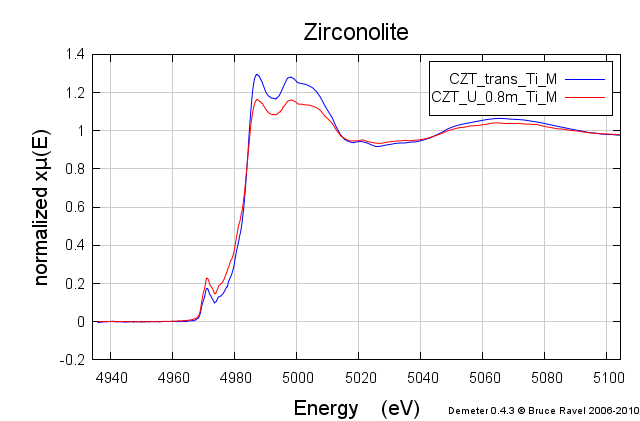
\includegraphics[width=0.9\linewidth]{images/zirc_xanes.png}

        Zirconolite CaZrTi$_2$O$_7$ {\color{Blue3}powder in
          transmission} and a {\color{Red2}sintered pellet in
          fluorescence}.
      \end{center}
    \end{column}
    \begin{column}{0.5\linewidth}
      \begin{center}
        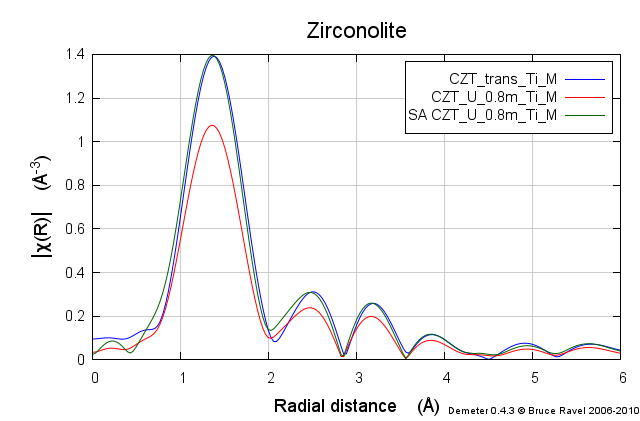
\includegraphics[width=0.9\linewidth]{images/zirc_chir.png}

        The data can be approximately corrected for the effect of
        self-absorption using \textsc{athena}.
      \end{center}
    \end{column}
  \end{columns}
  \begin{textblock*}{0.5\linewidth}(0pt,19.5\TPVertModule)
    \tiny%
    D.P.\ Reid, et al., Nuclear Instruments and Methods in Physics
    Research B, \textbf{268}:11-12, (2010) 1847
    \href{http://dx.doi.org/10.1016/j.nimb.2010.02.026}
    {\color{Purple4}DOI: 10.1016/j.nimb.2010.02.026}
  \end{textblock*}
\end{frame}

\begin{frame}[label=selfabs]
  \frametitle{Avoiding self-absorption}
  \begin{alertblock}{It is better to \textit{avoid} than to \textit{correct}!}
    The best approach is to prepare your sample in a way that will see
    a negligible self-absorption effect.
  \end{alertblock}

  \begin{itemize}
  \item Measure in transmission, if possible.
  \item Make your sample thin compared an absorption length.
  \item Make your sample dilute in absorber concentration.
  \item If possible, measure a standard that can be used to guide the
    self-absorption correction, as shown on the previous slide.
  \end{itemize}

  \begin{block}{Your sample \textit{is} your sample}
    Sometimes self-absorption cannot be avoided. $\ddot\frown$
  \end{block}
\end{frame}

\begin{frame}
  \frametitle{Dead time}

  \small
  When using an energy discriminating detector, data can be distorted
  due to ``pile-up'', which is due to photons arriving faster than the
  discriminating electronics can process them.
  \begin{columns}[T]
    \begin{column}{0.5\linewidth}
      \begin{center}
        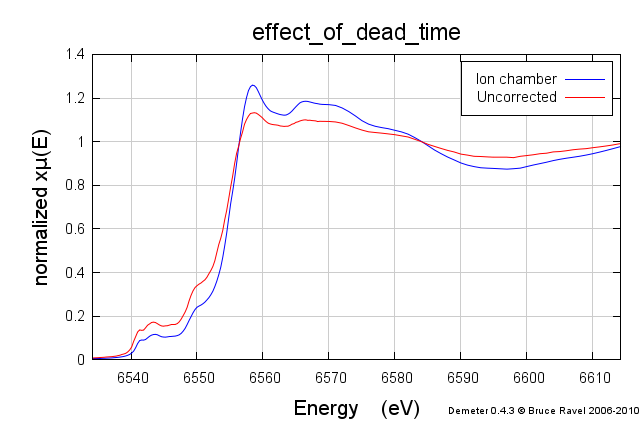
\includegraphics[width=0.9\linewidth]{images/deadtime.png}

        SrMnO$_3$ measured at a very high count rate with a
        {\color{Red2}Si-drift detector}, compared to data measured
        with {\color{Blue2}a Stern-Heald detector}.
      \end{center}
    \end{column}
    \begin{column}{0.5\linewidth}
      \begin{center}
        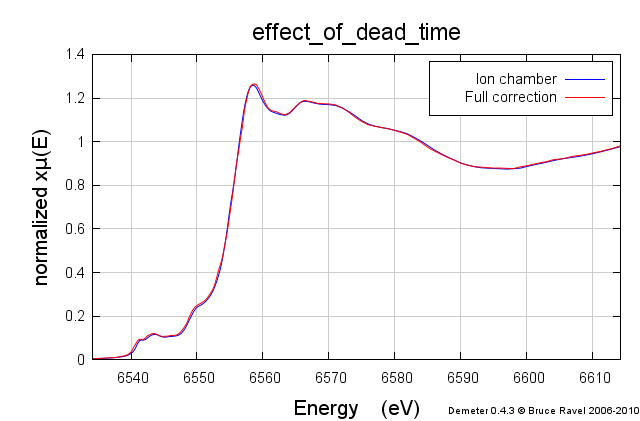
\includegraphics[width=0.9\linewidth]{images/deadtime_corrected.png}

        Data can be accurately corrected to restore the true measurement.
      \end{center}
    \end{column}
  \end{columns}
  \begin{textblock*}{0.5\linewidth}(0pt,18.5\TPVertModule) \tiny%
    \textit{Performance of a four-element Si drift detector for X-ray
      absorption fine-structure spectroscopy}, J. C. Woicik, B. Ravel,
    D. A. Fischer and W. J. Newburgh, J. Synchrotron Rad. (2010)
    \textbf{17}, 409-413,
    \href{http://dx.doi.org/10.1107/S0909049510009064}
    {\color{Purple4}DOI: 10.1107/S0909049510009064}
  \end{textblock*}
\end{frame}

\section[Fingerprinting]{Fingerprinting}

\begin{frame}
  \frametitle{Fingerprinting}
  \begin{block}{Fingerprint, \textit{tr.v.}}
    To identify by means of a distinctive mark or characteristic.
  \end{block}

  \small

  One of the most powerful uses of XANES data is to simply identify
  what is in front of the beam.

  Looking back at the Cr$^{III}$/Cr$^{VI}$ example, what might you say
  about the valence of the chromium contained in coal combustion residue?

  \begin{columns}[T]
    \begin{column}{0.45\linewidth}
      \begin{center}
        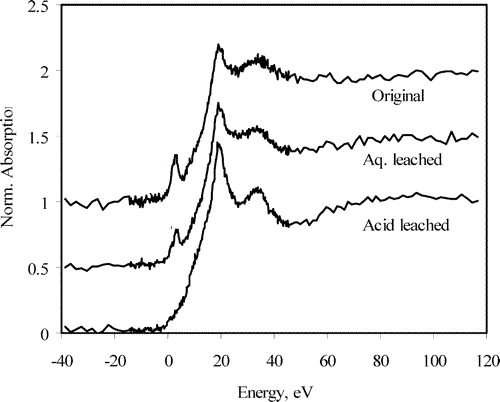
\includegraphics[width=0.8\linewidth]{images/cr_coal.png}
      \end{center}
    \end{column}
    \begin{column}{0.45\linewidth}
      \begin{center}
        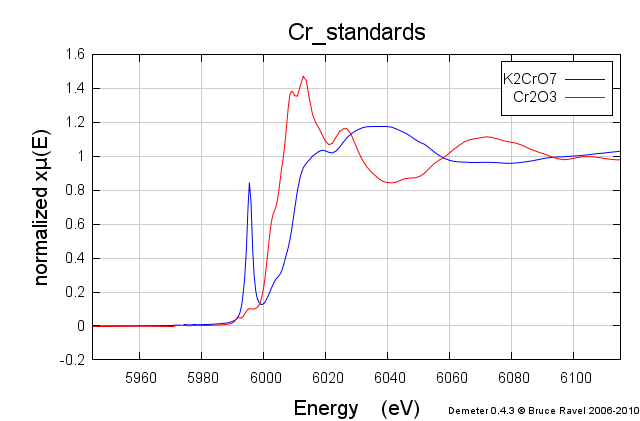
\includegraphics[width=0.9\linewidth]{images/Cr/Cr.png}
      \end{center}
    \end{column}
    \begin{column}{0.05\linewidth}
      \begin{center}
        {\color{Blue3}K$_2$CrO$_7$}\\
        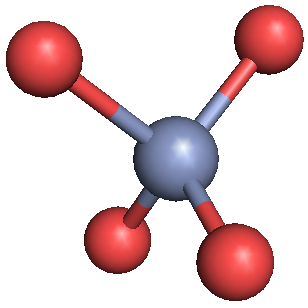
\includegraphics[width=\linewidth]{images/Cr/K2CrO7.png}\\[2ex]
        {\color{Red2}Cr$_2$O$_3$}\\
        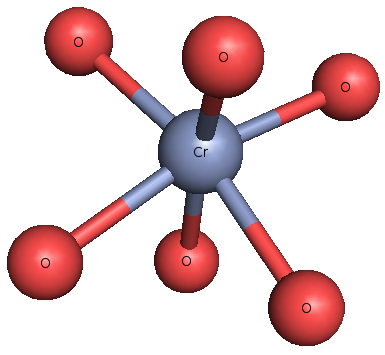
\includegraphics[width=\linewidth]{images/Cr/Cr2O3.png}
      \end{center}
    \end{column}
  \end{columns}

  \begin{textblock*}{0.5\linewidth}(0pt,19.25\TPVertModule)
    \tiny%
    \textit{Quantifying Hazardous Species in Particulate Matter
      Derived from Fossil-Fuel Combustion}, F.E.\ Huggins, et al.,
    Environ. Sci. Technol. (2004) \textbf{38}:6, 1836
    \href{http://dx.doi.org/10.1021/es0348748}
    {\color{Purple4}DOI: 10.1021/es0348748}
  \end{textblock*}
\end{frame}

\begin{frame}
  \frametitle{Categorizing spectra}
  
  In an study of Ti-containing standard materials, the different
  coordination environments were found to aggregate when plotting
  pre-edge peak height v. peak position.

  \begin{columns}
    \begin{column}{0.6\linewidth}
      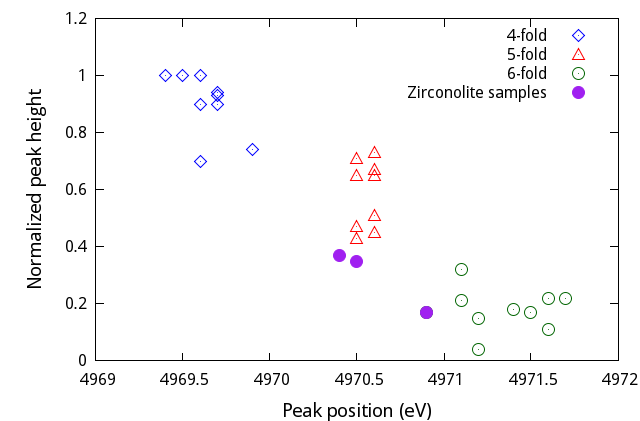
\includegraphics[width=\linewidth]{images/Farges/farges.png}
    \end{column}
    \begin{column}{0.4\linewidth}
      Here we see the data from the reference below along with Ti
      K-edge data from various Zirconolite (CaZrTi$_2$O$_7$) samples,
      including the one from the
      \hyperlink{selfabs}{\color{Purple4}self-absorption slide}.
    \end{column}
  \end{columns}

  \begin{textblock*}{0.52\linewidth}(0pt,19\TPVertModule) 
    \tiny%
    \textit{Coordination chemistry of Ti (IV) in silicate glasses and
      melts: I. XAFS study of titanium coordination in oxide model
      compounds }, Geochimica et Cosmochimica Acta, \textbf{60}:16,
    3023, 1996, \href{http://dx.doi.org/10.1016/0016-7037(96)00144-5}
    {\color{Purple4}DOI: 10.1016/0016-7037(96)00144-5}
  \end{textblock*}
\end{frame}

\begin{frame}
  \frametitle{XANES and disorder}

  The details of the XANES can often give information about structural
  disorder about the absorbing atom.
  
  \begin{columns}
    \begin{column}{0.4\linewidth}
      \begin{center}
        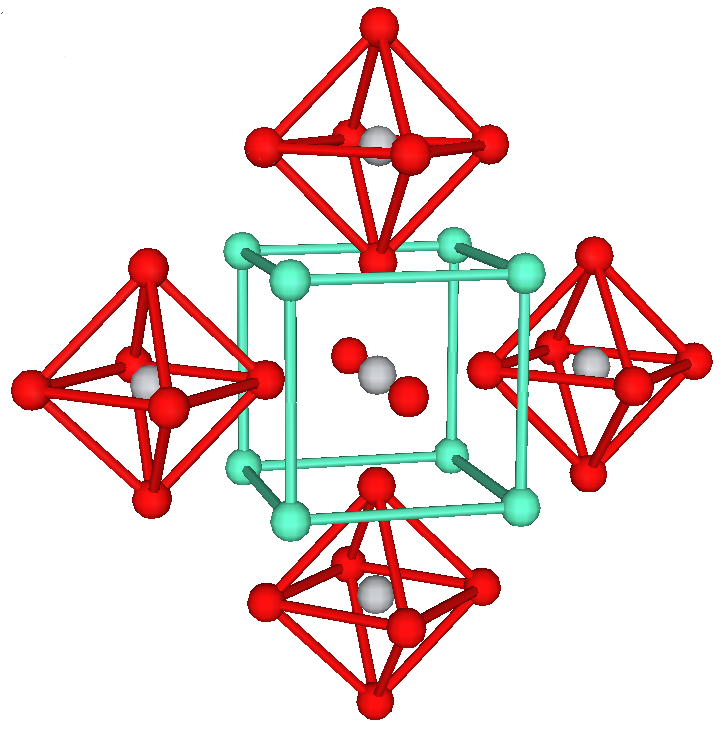
\includegraphics[width=0.6\linewidth]{images/perovskite.png}
      \end{center}
    \end{column}
    \begin{column}{0.6\linewidth}
      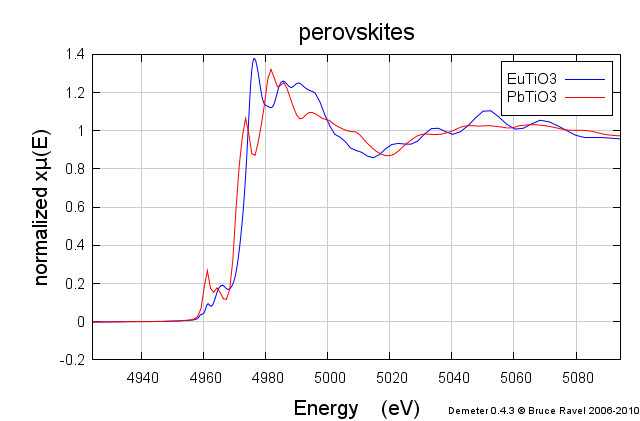
\includegraphics[width=\linewidth]{images/perov_xanes.png}
    \end{column}
  \end{columns}
  {\color{Blue3}EuTiO$_3$} is a true cubic perovskite.
  {\color{Red2}PbTiO$_3$} is a tetragonally distorted perovskite with
  substantial disorder in the oxygen octahedron.  Consequently, the
  pre-edge peak is much larger for {\color{Red2}PbTiO$_3$}.


  \begin{textblock*}{0.52\linewidth}(0pt,19\TPVertModule)
    \tiny%
    \textit{Local structure and the phase transitions of BaTiO$_3$}
    B. Ravel, E. A. Stern, R. I. Vedrinskii, V. Kraizman
    Ferroelectrics, \textbf{206}:1 (1998) 407,
    \href{http://dx.doi.org/10.1080/00150199808009173 }
    {\color{Purple4}DOI: 10.1080/00150199808009173 }
  \end{textblock*}
\end{frame}

\begin{frame}
  \frametitle{Why are disorder and the pre-edge peak related?}

  \begin{itemize}
  \item XAS is a dipole transition.  The photoelectron changes angular
    momentum by 1: $\ell\pm1$.
  \item For a K-edge spectrum, the initial state is \textit{s}:
    $\ell=0$.  Thus  the final state must be $\ell=1$.
  \item Ti has a filled \textit{p} shell but a completely empty
    \textit{d} shell.
  \item With centro-symmetry, as in a true perovskite, the \textit{p}
    and \textit{d} states cannot hybridize.  Broken symmetry leads to
    mixing of \textit{p} and \textit{d} states around the Fermi level.
  \item Disorder-driven admixture of \textit{d} character results in
    an enhanced pre-edge peak.
  \end{itemize}

\end{frame}
\section[Analysis]{Analysis Methods}

\begin{frame}
  \frametitle{Analysis}

  There are a number of ways to get quantitative results from XANES
  spectra:
  \begin{description}[Linear]
  \item[Linear Combination Fitting] ~\\Interpret data by comparison with
    standards
  \item[Peak Fitting] ~\\Fit Gaussian and Lorentzian line-shapes to the
    peaks in XANES data
  \item[Principle Components Analysis] ~\\Decompose an ensemble of data
    into a mathematical basis
  \item[Difference Spectra] ~\\Subtract one normalized spectrum from
    another 
  \end{description}

  \begin{block}{Software}
    \textsc{athena} is able to do all of these except for PCA.\\
    \textsc{SixPack} and other programs have good PCA implementations.
  \end{block}
\end{frame}

\subsection[LCF]{Linear Combination Fitting}

\begin{frame}
  \frametitle{LCF}

  \begin{block}{The working assumption of LCF}
    The spectrum from an unknown sample can be understood as a linear
    superposition of the spectra of two or more known samples.
  \end{block}

  That is:

  \begin{columns}
    \begin{column}{0.2\linewidth}
      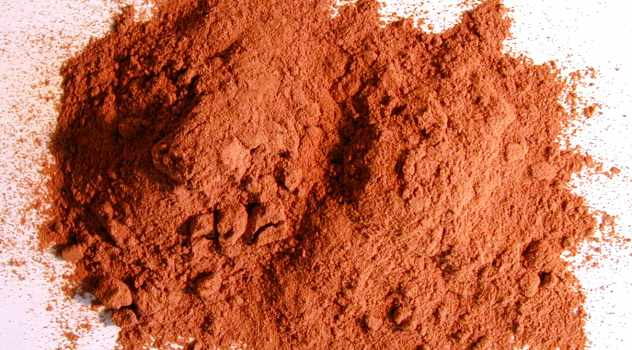
\includegraphics[width=\linewidth]{images/cinnamon_powder.jpg}
    \end{column}
    \begin{column}{0.03\linewidth}
      +
    \end{column}
    \begin{column}{0.2\linewidth}
      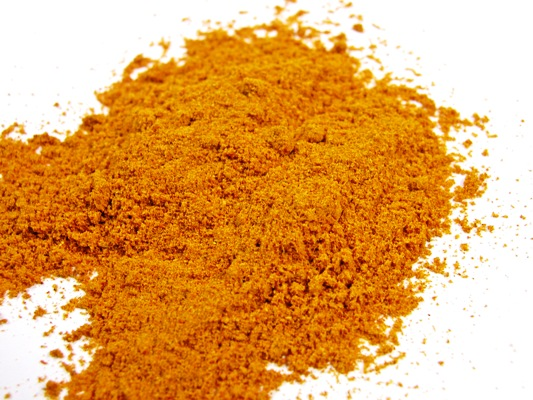
\includegraphics[width=\linewidth]{images/curry-powder.jpg} 
    \end{column}
    \begin{column}{0.03\linewidth}
      =
    \end{column}
    \begin{column}{0.2\linewidth}
      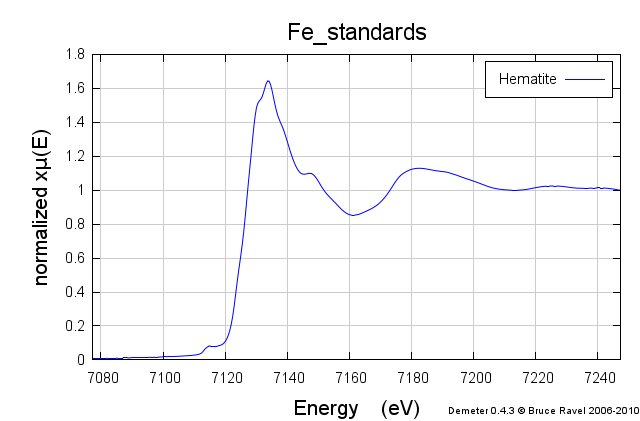
\includegraphics[width=\linewidth]{images/hematite.png} 
    \end{column}
    \begin{column}{0.03\linewidth}
      +
    \end{column}
    \begin{column}{0.2\linewidth}
      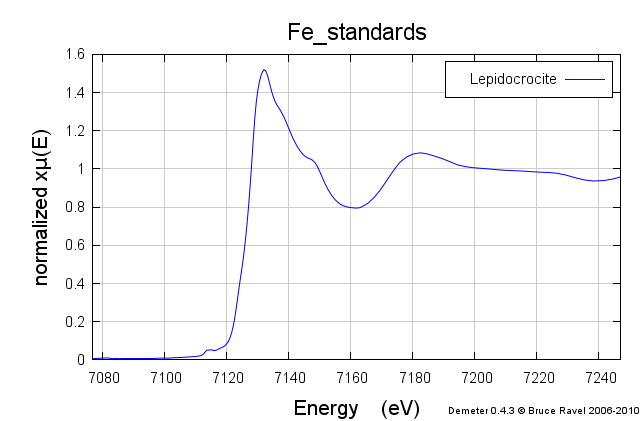
\includegraphics[width=\linewidth]{images/lepidocrocite.png}
    \end{column}
  \end{columns}

  \bigskip

  LCF requires:
  \begin{enumerate}
  \item A complete set of standards (i.e.\ every possible constituent)
  \item High quality measurements of each standard
  \item Data and standard are aligned to a common absolute energy grid
    and processed (i.e.\ normalization and background removal)
    consistently
  \end{enumerate}
\end{frame}



\begin{frame}
  \frametitle{Economic geology (I)}

  One way that gold deposits form is by having Au chloride fluids rise
  from the deep earth, wash over cyanobacteria colonies, and
  eventually reduce to metallic gold.

  \begin{columns}
    \begin{column}{0.5\linewidth}
      \includegraphics[width=\linewidth]{images/AuCl/aucl_exp.pdf}
    \end{column}
    \begin{column}{0.5\linewidth}
      We simulated this process at the beamline by exposing
      cyanobacteria to an Au$^{3+}$ solution and ``watching'' the
      evolution of the Au XAS from Au$^{3+}$ to Au$^0$.

      \begin{block}{Questions}
        \begin{itemize}
        \item What is the rate constant?
        \item Is there an intermediate species?
        \end{itemize}
      \end{block}
    \end{column}
  \end{columns}

  \begin{textblock*}{0.5\linewidth}(0pt,19\TPVertModule) 
    \tiny
    M. Lengke et el., \textit{Mechanisms of Gold Bioaccumulation by
      Filamentous Cyanobacteria from Gold(III)-Chloride Complex},
    Environ. Sci. Technol. \textbf{40}(20) p.~6304-6309. (2006)
  \end{textblock*}
\end{frame}
\begin{frame}
  \frametitle{Economic geology (II)}

  \begin{columns}[T]
    \begin{column}{0.5\linewidth}
      We see that \alert{7 minutes} after injection, the data strongly
      resemble the {\color{Blue3}Au$^{3+}$Cl}.  After
      {\color{Purple4}one week}, the data resemble
      {\color{Green4}Au metal}.
    \end{column}
    \begin{column}{0.5\linewidth}
      Over the course of the time series, the white line $\sim11921$
      shrinks while the bump $\sim11945$ grows, suggesting the
      reduction to Au metal.
    \end{column}
  \end{columns}

  \bigskip

  \begin{columns}[T]
    \begin{column}{0.5\linewidth}
      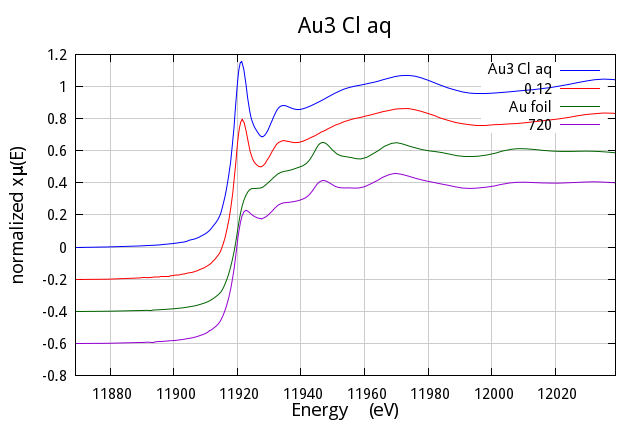
\includegraphics[width=\linewidth]{images/AuCl/aucl_data.png}
    \end{column}
    \begin{column}{0.5\linewidth}
      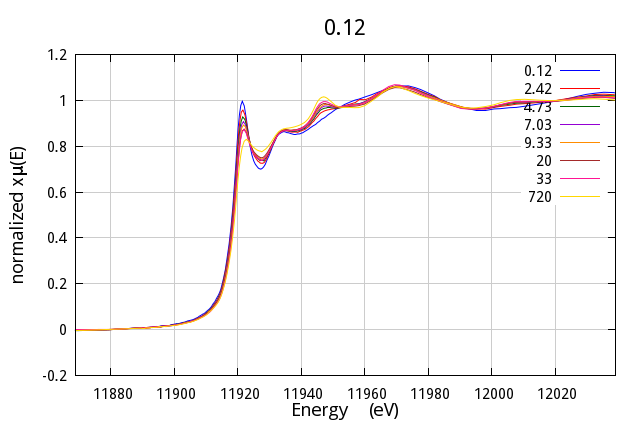
\includegraphics[width=\linewidth]{images/AuCl/aucl_time.png}
    \end{column}
  \end{columns}
  \begin{textblock*}{0.5\linewidth}(0pt,19\TPVertModule) 
    \tiny
    M. Lengke et el., \textit{Mechanisms of Gold Bioaccumulation by
      Filamentous Cyanobacteria from Gold(III)-Chloride Complex},
    Environ. Sci. Technol. \textbf{40}(20) p.~6304-6309. (2006)
  \end{textblock*}
\end{frame}
\begin{frame}
  \frametitle{Economic geology (III)}

  \begin{columns}[T]
    \begin{column}{0.5\linewidth}
      We can analyze these data as a linear combination of species,
      including {\color{Green4}Au$^{3+}$Cl}, {\color{Purple4}Au
        metal}, and {\color{Orange2}Au$^{1+}$ sulfide}.
    \end{column}
    \begin{column}{0.5\linewidth}
      We plot the contributions from these species as a function of
      time to see reaction rates.
    \end{column}
  \end{columns}

  \bigskip

  \begin{columns}[T]
    \begin{column}{0.5\linewidth}
      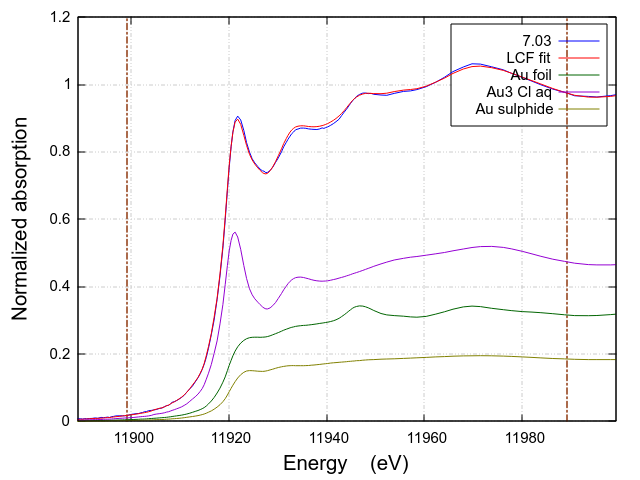
\includegraphics[width=\linewidth]{images/AuCl/aucl_lcf.png}
    \end{column}
    \begin{column}{0.5\linewidth}
      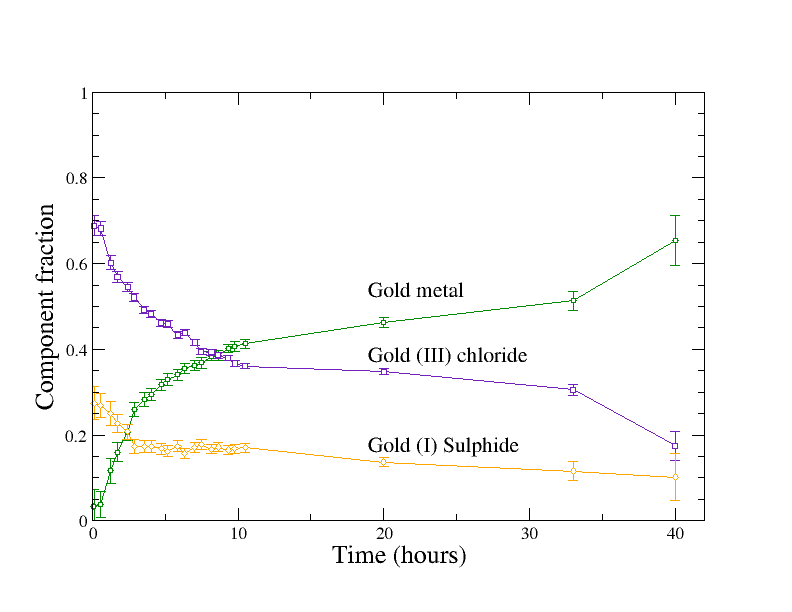
\includegraphics[width=\linewidth]{images/AuCl/aucl_results.png}
    \end{column}
  \end{columns}
  \begin{textblock*}{0.5\linewidth}(0pt,19\TPVertModule) 
    \tiny
    M. Lengke et el., \textit{Mechanisms of Gold Bioaccumulation by
      Filamentous Cyanobacteria from Gold(III)-Chloride Complex},
    Environ. Sci. Technol. \textbf{40}(20) p.~6304-6309. (2006)
  \end{textblock*}
\end{frame}





\subsection[Peak]{Peak Fitting}

\begin{frame}
  \frametitle{Peak fitting}

  \begin{block}{The working assumption of peak fitting}
    A spectrum can be meaningfully deconstructed into a set of
    step-like (atan or erfc) and peak (Gaussian, Lorentzian, Voight)
    functions.
  \end{block}

  \begin{columns}
    \begin{column}{0.4\linewidth}
      \begin{center}
        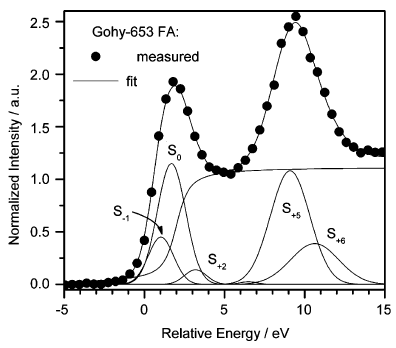
\includegraphics[width=0.9\linewidth]{images/S_peak.png}
      \end{center}
    \end{column}
    \begin{column}{0.6\linewidth}
      In this case, various Gaussians are interpreted as being the
      contributions from differently S valence states, with thiol and
      sulfonate dominating in a humic material from an aquifer in
      northern Germany.
    \end{column}
  \end{columns}

  This sort of analysis is most meaningful when performed across an
  ensemble of related data.  The drawback is that the physical
  significance of the line-shapes is sketchy, at best.

  \begin{textblock*}{0.52\linewidth}(0pt,19.25\TPVertModule)
    \tiny%
    \textit{Origin and mobility of fulvic acids in the Gorleben
      aquifer system}, T.\ Sch\"afer, et al., Organic
    Geochemistry, \textbf{36}:4, (2005) 567,
    \href{http://dx.doi.org/10.1016/j.orggeochem.2004.10.011}
    {\color{Purple4}DOI: 10.1016/j.orggeochem.2004.10.011}
  \end{textblock*}
\end{frame}

\subsection[PCA]{Principle Components Analysis}

\begin{frame}
  \frametitle{Principle Components (Factor) Analysis}

  \begin{block}{The working assumption of PCA}
    An ensemble of data represents a number of physical components
    that is equal to or smaller than the size of the ensemble.
  \end{block}

  \begin{enumerate}
  \item Decompose the ensemble of spectra into an orthogonal set of
    eigenvectors.  These are purely mathematical vectors that do not
    individually represent physical components of the data.
  \item When done correctly, the number of significant eigenvalues
    equals the number of physical components of the system.
  \item \textit{Target transforms} can be done to test potential
    physical components against the eigenvectors.
  \item Great care must be taken to align and normalize the data
    properly.  Any errors in data processing show up as additional
    non-negligible eigenvectors.
  \item \textsc{SixPack} has a nice implementation.  \textsc{athena}
    does not (yet).
  \end{enumerate}

  \begin{textblock*}{0.52\linewidth}(0pt,19.25\TPVertModule)
    \tiny%
    S.R.\ Wasserman, J.\ Phys. IV France (1997) C2-203-C2-205; S.R.\
    Wasserman et al., J.\ Synchrotron Rad.\ (1999) 6, 284-286;
    references therein
  \end{textblock*}
\end{frame}

\subsection[Diff]{Difference Spectra}

\begin{frame}
  \frametitle{Difference Spectra}

  \begin{block}{Difference spectra}
    Subtract one spectrum from another.
  \end{block}

  \small

  \begin{columns} [T]
    \begin{column}{0.6\linewidth}
      The most common use is for X-ray Magnetic Circular Dichroism
      (XMCD)

      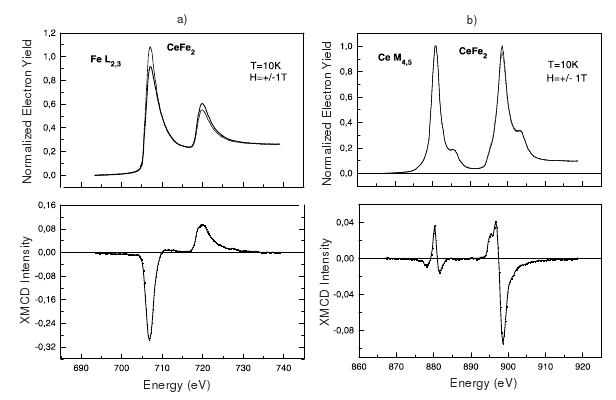
\includegraphics[width=0.9\linewidth]{images/xmcd.png}

      The areas under the difference spectra tell you about moment and
      magnetic ordering.
    \end{column}
    \begin{column}{0.4\linewidth}
      Difference spectra can also be used to highlight a subtle change
      in a data sequence.

      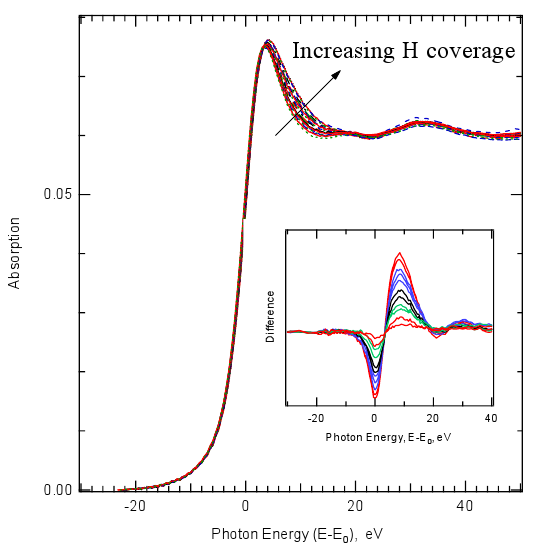
\includegraphics[width=0.9\linewidth]{images/HPt.png}

      Here, Pt nanoparticles are being covered with H.
    \end{column}
  \end{columns}

  \begin{textblock*}{0.52\linewidth}(0pt,19.25\TPVertModule)
    \tiny%
    \textit{X-ray magnetic circular dichroism study on CeFe2},
    A. Delobbe, et al., Europhys.\ Lett.\ \textbf{43} 320 (1998),
    \href{http://dx.doi.org/10.1209/epl/i1998-00359-2}
    {\color{Purple4}DOI: 10.1209/epl/i1998-00359-2}; Pt data courtesy
    of Simon Bare
  \end{textblock*}
\end{frame}

\section[Theory]{Using Theory}

\begin{frame}
  \frametitle{Feff}
  
  \begin{columns}
    \begin{column}{0.55\linewidth}
      \textsc{feff} is a widely popular, real-space, multiple
      scattering code used for XANES, EXAFS, and other spectroscopies.
      It is fully integrated into \textsc{artemis} and not hard to use
      on its own.  A GUI exists.

      \medskip

      Simulating XANES data is not hard, although much thought needs
      to go into the cluster and the parameters to make the
      calculation useful for comparison with real data.  \textsc{feff}
      is a single electron, dipole approximation code ---
      multi-electron excitations, quadrupole contributions to the
      XANES, and multiplet effects are not calculated.

      \medskip

      Works on all computer platforms.
    \end{column}
    \begin{column}{0.45\linewidth}
      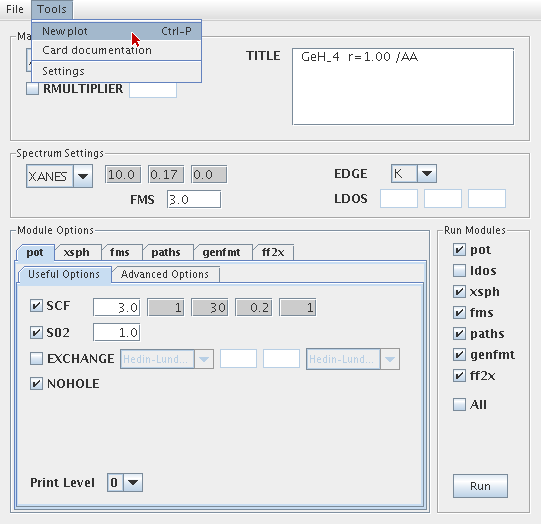
\includegraphics[width=0.9\linewidth]{images/jfeff.png}
    \end{column}
  \end{columns}


  \bigskip

  \href{}
  {\color{Purple4}\textsc{feff} homepage: http://leonardo.phys.washington.edu/feff/}

\end{frame}

\begin{frame}
  \frametitle{Multiplets}
  \begin{columns}
    \begin{column}{0.65\linewidth}
      One electron codes can fail for systems with strong overlap
      between the core and valence states.  Transition metal L edges
      are a good example: strong overlap between the 2p and 3d bands.

      \bigskip

      Here is an Fe L$_{2,3}$ calculation for a low-spin ferric
      complex.  The quantum chemical calculation is made to find the
      many discrete states of the system and an instrumental/lifetime
      broadening is applied.

      \bigskip

      \href{http://www.anorg.chem.uu.nl/people/staff/FrankdeGroot/ttmultiplets.htm}
      {\color{Purple4}One popular multiplet code is by Frank de Groot.}  Windows only.
    \end{column}
    \begin{column}{0.35\linewidth}
      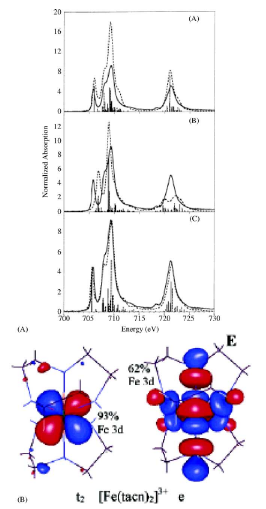
\includegraphics[width=0.9\linewidth]{images/multiplet.png}
    \end{column}
  \end{columns}
  
  \begin{textblock*}{0.52\linewidth}(0pt,19.25\TPVertModule)
    \tiny%
    \textit{Multiplet effects in X-ray spectroscopy},
    F.\ de Groot, Coord.\ Chem.\ Rev.\ \textbf{249}:1-2 31 (2005),
    \href{http://dx.doi.org/10.1016/j.ccr.2004.03.018}
    {\color{Purple4}DOI: 10.1016/j.ccr.2004.03.018}
  \end{textblock*}
\end{frame}

\begin{frame}
  \frametitle{FDMNES}
  The Schr\"odinger equation is solved in a discrete form on a
  three-dimensional grid using a finite difference method.  From this,
  many calculations are possible, including XAS, XES, RIXS, anomalous
  scattering, and others.

  \bigskip
  
  This approach avoids certain shortcomings of \textsc{feff}8 in
  highly non-centro-symmetric systems.

  \bigskip
  
  Windows and linux.

  \bigskip

  \href{http://www.neel.cnrs.fr/spip.php?article876}
  {\color{Purple4}FDMNES homepage:
    http://www.neel.cnrs.fr/spip.php?article876}


  \begin{textblock*}{0.52\linewidth}(0pt,19.25\TPVertModule)
    \tiny%
    \textit{X-ray absorption near-edge structure calculations beyond
      the muffin-tin approximation}, 
    Y.\ Joly, Phys.\ Rev. B \textbf{63}  125120 (2002),
    \href{http://dx.doi.org/10.1103/PhysRevB.63.125120}
    {\color{Purple4}DOI: 10.1103/PhysRevB.63.125120}
  \end{textblock*}
\end{frame}

\begin{frame}
  \frametitle{FitIt}
  \begin{columns}
    \begin{column}{0.5\linewidth}
      Fit XANES spectra by multidimensional interpolation using
      \textsc{feff} or \textsc{fdmnes} calculations.

      \smallskip

      This software helps you set up the calculations and parametrize
      your fit.

      \smallskip

      Windows only.
    \end{column}
    \begin{column}{0.5\linewidth}
      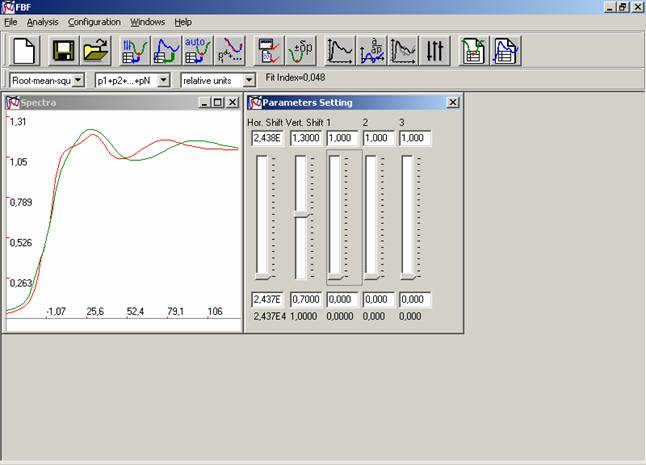
\includegraphics[width=0.9\linewidth]{images/fitit_2.jpg}      
    \end{column}
  \end{columns}

  \bigskip

  \href{http://www.nano.sfedu.ru/fitit.html}
  {\color{Purple4}FitIt homepage: http://www.nano.sfedu.ru/fitit.html}
\end{frame}

\begin{frame}
  \frametitle{Using theory effectively}
  \begin{columns}
    \begin{column}{0.4\linewidth}
      \begin{center}
        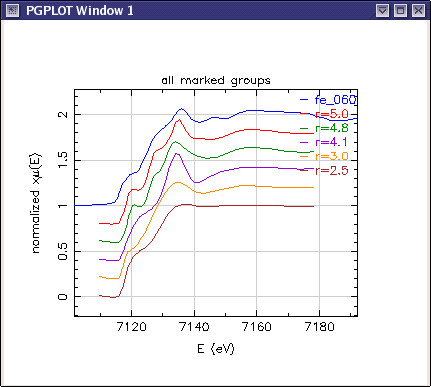
\includegraphics[width=0.9\linewidth]{images/xanes_convergence.png}
      \end{center}
    \end{column}
    \begin{column}{0.6\linewidth}
      Convergence in cluster size.  Near the edge, the mean free path
      of the photoelectron is quite large.  The only way to know the
      proper cluster size is the do the calculations.
    \end{column}
  \end{columns}

  \begin{columns}
    \begin{column}{0.4\linewidth}
      \begin{center}
        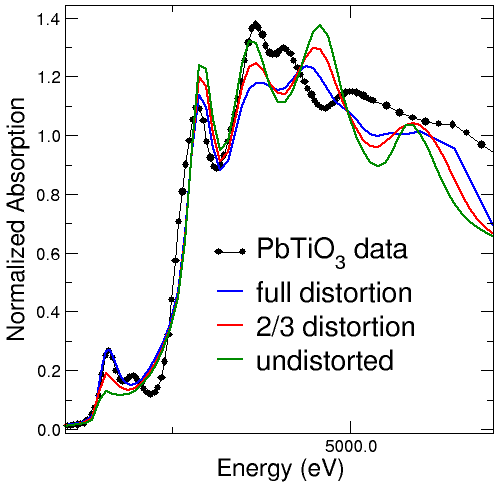
\includegraphics[width=0.9\linewidth]{images/pto.png}
      \end{center}
    \end{column}
    \begin{column}{0.6\linewidth}
      Often the theory is an imperfect match to the data, but a
      sequence of calculations shows a same trend that can be related
      to the data.

      In this case, a sequence of calculations on PbTiO$_3$ shows the
      relation between pre-edge peak and amount of distortion.
    \end{column}
  \end{columns}
\end{frame}

\section{Summary}

\begin{frame}
  \frametitle{Summary}
  \begin{description}
  \item[XANES is a much larger signal than EXAFS] Good XANES spectra
    can be collected at lower concentrations and with
    less-than-perfect samples.
  \item[XANES is easier to crudely interpret than EXAFS] In many
    cases, XANES can be a fingerprinting tool.  For many systems, the
    XANES analysis using known spectra from model compounds is
    sufficient.
  \item[XANES is harder to fully interpret than EXAFS] The exact
    physical and chemical interpretation of all spectral features is
    still difficult to do accurately, precisely, and reliably.  This
    situation is improving...
  \end{description}
\end{frame}

\begin{frame}
  \frametitle{Notes}
\end{frame}

\end{document}

%%% Local Variables:
%%% mode: latex
%%% TeX-master: t
%%% End:
